\chapter{Einbettung in Gaia-X kompatible Cloud}
\label{chapter:gaia-x-einbettung}
Gaia-X ermöglicht und fördert die Bildung von sogenannten \emph{Federations}.
Federations werden als eingeständige Ökosysteme beschrieben, in denen sich einzelne Teilnehmer zusammenschließen könnnen,
um Services innerhalb oder auch außerhalb der Federation anzubieten, um Teilnehmern einen Mehrwert zu bieten.
Gaia-X operiert nicht, wie alleinstehende Cloud-Providerfirmen, selbst auf dem Markt, sondern erstellt
Software Komponenten zur Erstellung eines förderalisierten Systems in dem mehrere Teilnehmer
untereinander kommunizieren und interagieren können \cite{GXFS2021}.
Als einer der ersten Testimplementationen für Gaia-X gilt die Pluscloud Open,
welche auf Basis des Open Source Projekts \ac{SCS} läuft.
Zum Zweck dieser Arbeit wurde eine zeitlich begrenzte Testlizenz bereitgestellt,
welche die Möglichkeit bietet, die in dieser Arbeit erstellte Referenzimplementation
in einer Gaia-X kompatiblen Umgebung zu testen.


\section{Erstellung der Testinfrastruktur}
\label{sec:gaia-x-einbettung:erstellung-testinfra}
Bei der Erstellung der Testinfrastruktur kam es zu einigen Einschränkungen im Vergleich zu bereits etablierten Hyperscaler Clouds,
da zum Zeitpunkt der Thesis nur Infrastruktur Services wie Netzwerke, DNS, \acp{VM} und Speicher
und kein Managed Kubernetes Service zur Verfügung stehen.
Durch die unterliegende Architektur des Gaia-X Providers kann bereits etablierte freie Software
im Cloud Umfeld genutzt werden, um die Bereitstellung eines Clusters zu ermöglichen.
Hierbei wurde das Tool \textbf{Kubespray}\footnote{\href{https://github.com/kubernetes-sigs/kubespray}{Kubespray}} genutzt,
welches mit Hilfe der Konfigurationssoftware \textbf{Ansible} und dem \ac{IaC} Tool \textbf{Terraform}
\acp{VM}, Netzwerk und Sicherheitsgruppen für die Kubernetes Knoten erstellt.

Aufgrund der zeitlichen Begrenzung von 30 Tagen der Testlizenz, wurde jedoch noch eine lokal
testbare Version der Openstack Services erstellt, welche Plusserver nutzt.
Hierbei werden alle benötigen Services in Containern bereitgestellt, welche auf der Entwicklungs-
plattform betrieben werden können.
Somit kann die Cloudunabhängigkeit von Kubernetes zum Vorteil für Entwickler genutzt werden.


\section{Bereitstellung im Gaia-X Katalog}
\label{sec:gaia-x-einbettung:gaia-x-katalog}
Gaia-X definiert als Standard einen sogenannten Katalog, in dem Federations Services registrieren können
und Endnutzer mittels Suchalogrithmen einen Service für ihre Bedürfnisse finden können.
Im Katalog bereitgestellte Services müssen den Nutzer informieren, welche Eigenschaften der jeweilige Service besitzt.
Dadurch können Endnutzer auswählen, welche Services in welcher Region und zu welchen Umständen sie nutzen möchten.
Dieses Prinzip wird in Gaia-X \emph{Self-Description} genannt. Self-Descriptions werden mittels JSON-LD dargestellt, ein
leichtgewichtiges \emph{Linked Data} Format \cite{Eggers2020}.

\begin{figure}
  \centering
  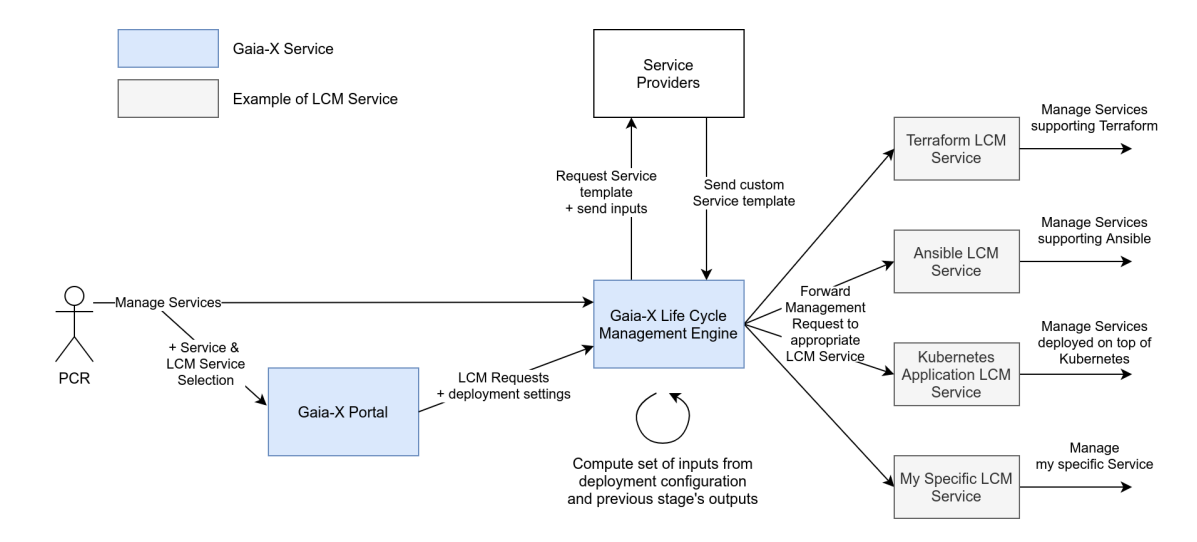
\includegraphics[width=\textwidth]{gfx/chapters/4_gaia-X/orchestration_overview.png}
  \caption{High Level Übersicht für Gaia-X Service Bereitstellung}
  \source{\cite{ORC2021}}
  \label{fig:gaia-x-orchestration-overview}
\end{figure}

In \ref{fig:gaia-x-orchestration-overview} wird die Kommunikation innerhalb Gaia-X Akteuren
zur Bereitstellung von Services in Gaia-X dargestellt.
Die \ac{LCM} Engine dient als Einstiegspunkt für Kommunikation mit dem Endnutzer. Jegliche Verwaltungsanfragen
für Services werden an sie gestellt. Die Engine verteilt daraufhin diese Anfragen
an den jeweiligen Bereitstellungsservice anhand der Auswahl des Nutzers.
Im Architekturbild übernimmt die in dieser Arbeit erstellte Referenzimplementation
den Teil des \emph{Kubernetes Application LCM Services}, wobei der \ac{LCM} Service die
Komponente des Rocket API Service entspricht.
Während der Auswahl von Gaia-X Services ist der Nutzer verantwortlich für die Wahl des \ac{LCM} Services.
Hierbei generiert das Portal eine Liste von möglichen Bereitstellungstechnologien,
weshalb jeder Service in einer \emph{Self-Description} angeben muss, welche Technologien den Service
verwalten sowie bereitstellen (Bereitstellungstechnologien) können.

Um die Konfiguration eines Services zu gewährleisten, muss der Anbieter eines Services eine Auswahl
an erforderlichen Eingaben, welche erforderlich für die Bereitstellung sind, sowie Standardparameter definieren.
Im Fall des Rocket Services werden die Eingaben mithilfe der definierten gRPC API bereitgestellt.
Der Nutzer des Services muss vor der Erstellung des Services eine Bereitstellungskonfiguration erstellen,
welche entweder mittels direktem Aufruf an die \ac{LCM} Engine oder dem Gaia-X Portal erstellt werden kann \cite{ORC2021}.

\begin{figure}[h]
  \centering
  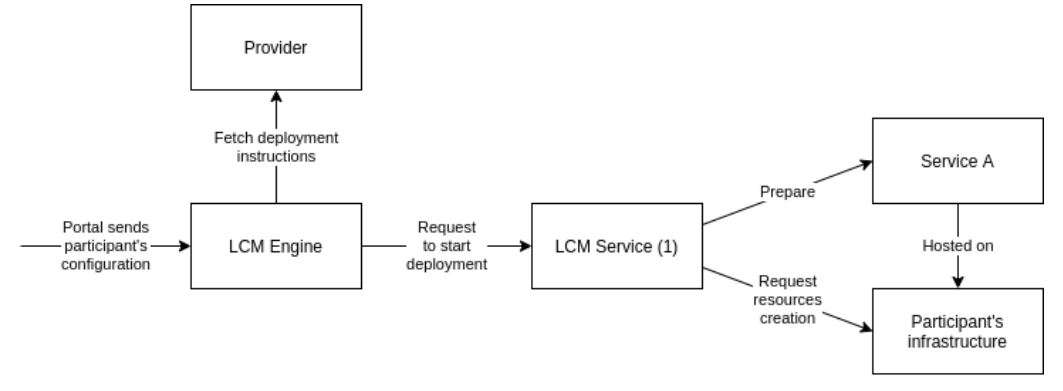
\includegraphics[width=\textwidth]{gfx/chapters/4_gaia-X/example_deployment.png}
  \caption{Beispiel einer Servicebereitstellung}
  \source{\cite{ORC2021}}
  \label{fig:gaia-x-example_deployment}
\end{figure}
Abbildung \ref{fig:gaia-x-example_deployment} verdeutlicht dieses Prinzip anhand eines Beispiels.
Ein Endnutzer übergibt seine gewünschte Konfiguration des Service A via Gaia-X Portal an die \ac{LCM} Engine weiter.
Service A kann dabei allerdings nicht mit allen LCM Services bereitgestellt werden,
sodass der Nutzer sich für den \emph{\ac{LCM} Service (1)} entscheidet.
Die Engine fragt beim Provider nach der Bereitstellungsanweisung für den Service an,
welche nach Zusammenführung mit der Nutzerkonfiguration an den \ac{LCM} Service weitergeleitet wird.
Der \ac{LCM} Service sorgt für die tatsächliche Bereitstellung des Service A
und gibt den Zugriffspunkt für den Service an die Engine zurück \cite{ORC2021}.
